% hacer una macro para \emph{place \& route}
\chapter{Flujo de Diseño Físico}
\section{Introducción}
\begin{figure}[h]
\centering
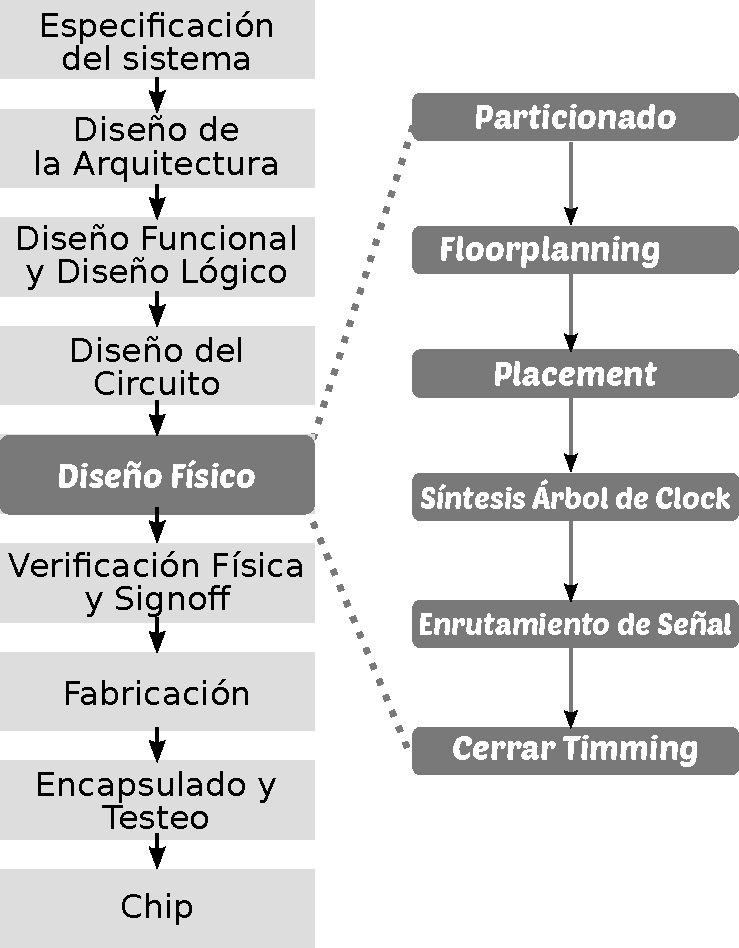
\includegraphics[scale=0.7]{figuras/DisenioFisico.pdf}
  \caption{Flujo de diseño Físico}
  \label{fig:diseñoFisico}
\end{figure}


\section{Relevamiento, comparación y selección de las herramientas disponibles}
\paragraph{Criterios para la selección}
\begin{itemize}
\item Desarrollo activo y que exista una comunidad de usuarios que brinden soporte
\item Mayor cantidad de herramientas integradas
\item Flexibilidad para importar y exportar datos. 
\item Design kits disponibles para la tecnología seleccionada.
\item Diseño físico a partir de la descripción estructural en VHDL\footnote{Condición necesaria ya que el resultado de nuestro diseño en el capítulo \ref{diseñoDigital} es una descripción estructural en VHDL.}.
\end{itemize}

La tecnología que se usará para fabricar es TSMC~180~nm\footnote{http://www.mosis.com/vendors/view/tsmc/018}.
Luego de una inspección de esos criterios, las herramientas candidatas que cumplen con esos criterios definidos son:

\begin{description}
\item[Alliance VLSI CAD System\footnote{Descripción extraída del sitio}]Alliance es un conjunto de herramientas libres, y librerías portables para el diseño de VLSI. Incluye un compilador vhdl y un simulador, herramientas de síntesis de lógica, y herramientas de \emph{place \& route} automáticas. Brinda un conjunto completo de librerías CMOS portables.

\item[Electric VLSI Design System] Es un sistema de Automatización de Diseño Electrónico. En un entorno integrado muy flexible que permite la descripción del circuito de varias formas (esquemáticos, VHDL, Layout, generadores de ROM y MOSIS PLA)   

\end{description}

%Open-Source VLSI CAD Tools: A Comparative Study



%Summary
%Alliance is a complete set of free CAD tools and portable libraries for VLSI design. It includes a VHDL compiler and simulator, logic synthesis tools, and automatic place and route tools. A complete set of portable CMOS libraries is provided, including a RAM generator, a ROM generator and a data-path compiler. Alliance is the result of more than ten years effort spent at ASIM department of LIP6 laboratory of the Pierre et Marie Curie University (Paris VI, France). Alliance has been used for research projects such as the 875 000 transistors StaCS superscalar microprocessor and 400 000 transistors IEEE Gigabit HSL Router. You are kindly requested to mention " Designed with alliance (c) LIP6, Université Pierre et Marie Curie" so as to spread the word about "alliance CAD system" and its development team. Alliance provides CAD tools covering most of all the digital design flow:
%VHDL Compilation and Simulation
%Model checking and formal proof
%RTL and Logic synthesis
%Data-Path compilation
%Macro-cells generation
%Place and route
%Layout edition
%Netlist extraction and verification
%Design rules checking alliance is listed among Fedora Electronic Lab (FEL) packages.
%Supported Fedora branches



\section{Selección de las Celdas estándar}\label{celdasEstandars}
El resultado de la síntesis que realizamos en el capítulo \ref{diseñoDigital} es un netlist VHDL que contiene sólo compuertas lógicas. Estas son compuertas lógicas abstractas, es decir que nuestro circuito fué mapeado a un conjunto finito de funciones logicas como las \verb.and., \verb.or., \verb.xor., \verb.xnor., etc.

Ahora es necesario mapear estas funciones lógicas a compuertas lógicas reales, que serán tambien un conjunto finito de compuertas, pero con dimensiones físicas definidas, y con una caracterización de su funcionamiento real. Estas compuertas lógicas se denominan celdas estándards, que se diseñan específicamente para la tecnología de fabricación que hayamos definido usar. Por cada función lógica existen distintas versiones para poder manejar distintas capacidades. 

Caraterización de las celdas: Se realizan simulaciones analógicas de un netlist de estas celdas, donde variando paramétricamente la carga (capacitiva) de salida y el tiempo de crecida y caída ($t_r$ y $t_f$) de la entrada, se obtiene el retardo de propagación, tiempo de crecida y de bajada de la salida y la disipación de potencia.


% Dibujo de una XOR en netlist mapeado a una XOR en layout.

\begin{figure}[h]
\centering
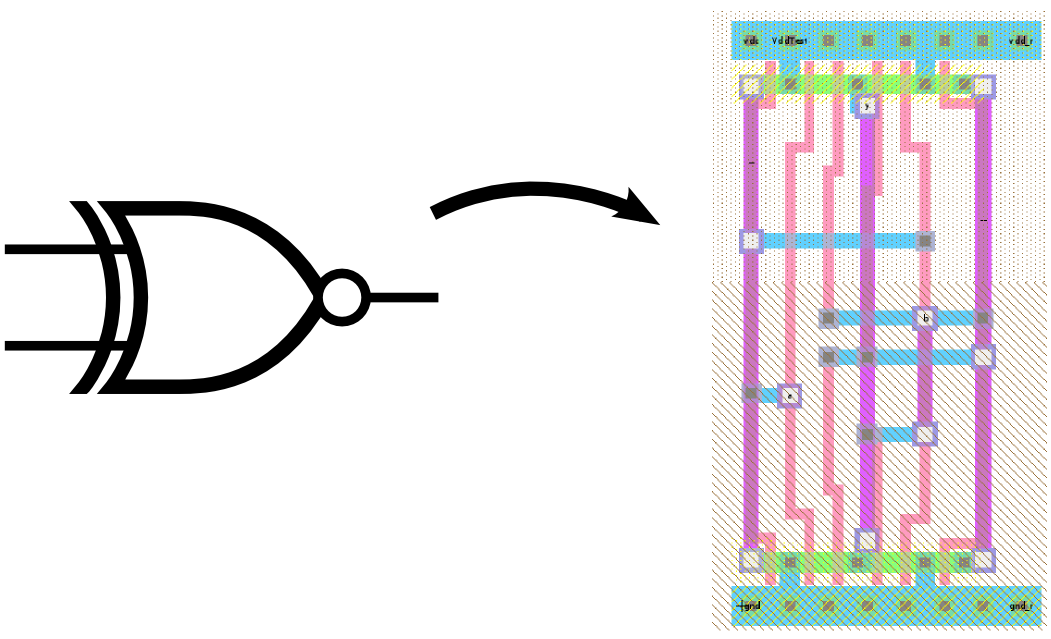
\includegraphics[scale=0.7]{figuras/map-xnor.png}
  \caption{Mapeo de funciones lógicas a celdas estándars}
  \label{fig:map-xnor}
\end{figure}

Es común elegir las celdas estándars según el tipo de aplicación a desarrollar. Existen celdas estandars que fueron diseñadas para bajo consumo, o alta velocidad, o de mínima área. También existe la posibilidad de diseñar celdas que busquen la mejor relación velocidad-consumo-area que puedan ser utilizadas en muchas aplicaciones. En circuitos integrados para sistemas alimentados a batería se intentará utilizar las celdas de menor consumo y evitar siempre que sea posible las de mayor velocidad, en función del presupuesto de potencia disponible para el mismo.

En nuestro caso, seleccionamos una librería de celdas estándars diseñadas para tamaño mínimo de canal n, y p. %Una referencia al Rabaey es necesaria? 
Otra característica de la librería es la distancia entre el riel de VSS hasta el riel de VDD. Esta distancia es de 117 $\lambda$ (En nuestra tecnología de 180~$\mathrm{nm}$, el valor de lambda es: $\lambda = 100~\mathrm{nm}$), lo cual permite el ruteo horizontal de 16 pistas de metal por encima de las celdas, con metal 3 hasta capas superiories.

 

%http://cmosedu.com/cmos1/electric/electric.htm
% “Tiny-Chip” padframes [1.5 mm x 1.5 mm]

\section{Ubicación y Cableado (\emph{Place \& Route})}
Partimos desde la descripción estructural\footnote{El resultado de la síntesis hecha con lava es un netlist a nivel de compuerta, listo para ser usado por una herramienta de \emph{place \& route}Gate-level netlist vhdl.} del vhdl que producimos en el capítulo \ref{diseñoDigital}. De \emph{Electric} usaremos la herramienta llamada \emph{Silicon Compiler}, que se encarga de ubicar y conectar las celdas según el archivo vhdl. En el apéndice \ref{vhdlNetlist} mostramos el resultado de sintetizar a compuertas nuestro circuito. Las compuertas que se usan son compuertas lógicas genéricas, aún podemos modificar este netlist primero para hacer optimizaciones lógicas, que en nuestro caso esto no es conveniente ya que hemos elegido la arquitectura para lograr la mejor relación de compromiso entre velocidad y menor interconectividad. Otra optimización a realizar es eligiendo la fuerza de la celda.



\emph{place \& route}



Arquero para que este archivo pueda ser usado con Electric fué necesario hacer algunas modificaciones:
\begin{enumerate}
\item Reemplazar los nombres de las instancias de las celdas estandards que  seleccionamos en la sección \ref{celdasEstandars} y \emph{Electric} utilizará.
\item En la parte del vhdl que comienza la descripción estructural es necesario agregar las celdas estandards que serán utilizadas en el circuito.
\item Quitar todas las instancias de \verb|wire port map (...)| volviendo a conectar lo que queda desconectado al quitar estas instancias.
\end{enumerate}  
Estas tareas las realizamos modificando el código del programa de lava que crea el netlist vhdl llamado \verb|VhdlNew.hs|, y con un script\footnote{Adjuntamos el script en el apéndice \ref{scriptPerl}} en perl que es lanzado desde el mismo.
\subsection{Métricas de Calidad de un circuito digital}

Para cuantificar la calidad de un circuito, podemos analizar un circuito desde diferentes perspectivas: Costo, funcionalidad, robustez, performance y consumo de energía. Tomaremos estas dos últimas métricas, mas la del área (propiedad que define el costo) del circuito, para realizar la comparación entre las distintas arquitecturas analizadas.

\subsubsection{Performance}
El término performance puede representar distintas métricas, según desde qué perpectiva se esté realizando el análisis. Pero si nos enfocamos puramente en el diseño, la performance se define usualmente\cite{rabaey2003} como la duración del período del clock (\emph{clock cycle time}) o su frecuencia (\emph{frecuencia del clock}). El valor mínimo de período de clock que pueda ser usado para una tecnología y un diseño dado, está definido por múltiples factores, como el tiempo que le toma a las señales propagarse a travez de la lógica, el tiempo que lleva entrar y salir los datos de los registros, la incerteza de llegada del reloj (\emph{clock uncertainty}). Pero el núcleo de todo el análisis de performance reside en la performance de una sola compuerta.

El retardo de propagación $t_p$ de una compuerta define cuan rápido responde un circuito a un cambio en su(s) entrada(s). Expresa el retardo experimentado por una señal cuando pasa a travez de una compuerta. Medido entre el 50\% del punto de transisción de entrada la señal de entrada y salida, como mostramos en la figura \ref{propagationDelay}, correspondiente al tiempo de propagación de una compuerta inversora. Ya que el tiempo de propagación es distinto según el flanco de entrada, se definen 2 tiempos de propagación. El $t_{pLH}$ es el tiempo de respuesta de una compuerta  para una transición de la salida desde bajo a alto, mientras que $t_{pHL}$ se refiere a el tiempo para una transición de la salida desde alto a bajo. El retardo de propagación $t_p$ se define como el promedio de estos dos.
$$ t_p = \frac{t_{pLH} + t_{pHL}}{2} $$

El retardo de propagación depende también de otros factores, como la pendiente de las señal de entrada, que depende de la señal de entrada que llega al circuito. Para cuantificar esta entrada, se usa el tiempo de crecida y de bajada $t_r$ y $t_f$. Este tiempo se especifica entre el \%10 y \%90 (o \%20 y \%80, o \%30 y \%70), como se muestra en la figura \ref{propagationDelay}. Estos tiempos simplemente nos dicen cuan rápido cambia de estado la señal de entrada.

Para poder comparar la performance de distintas tecnologías, se busca un circuito que no incluya parámetros como el fan-in o fan-out, capacidad de salida, etc. Por ello, el circuito que es un estandard de facto para medir el tiempo de propagación, es el oscilador anillo (\emph{ring oscillator}), que es un número impar de inversores conectados en serie, y la salida se vuelve a conectar a la entrada. Este circuito oscilla espontaneamente, a una frecuencia de $T = 2 \times t_p \times N$, con $N$ el número de inversores en la cadena.

\begin{figure}[h!]
\vspace{-5pt}
  \centering
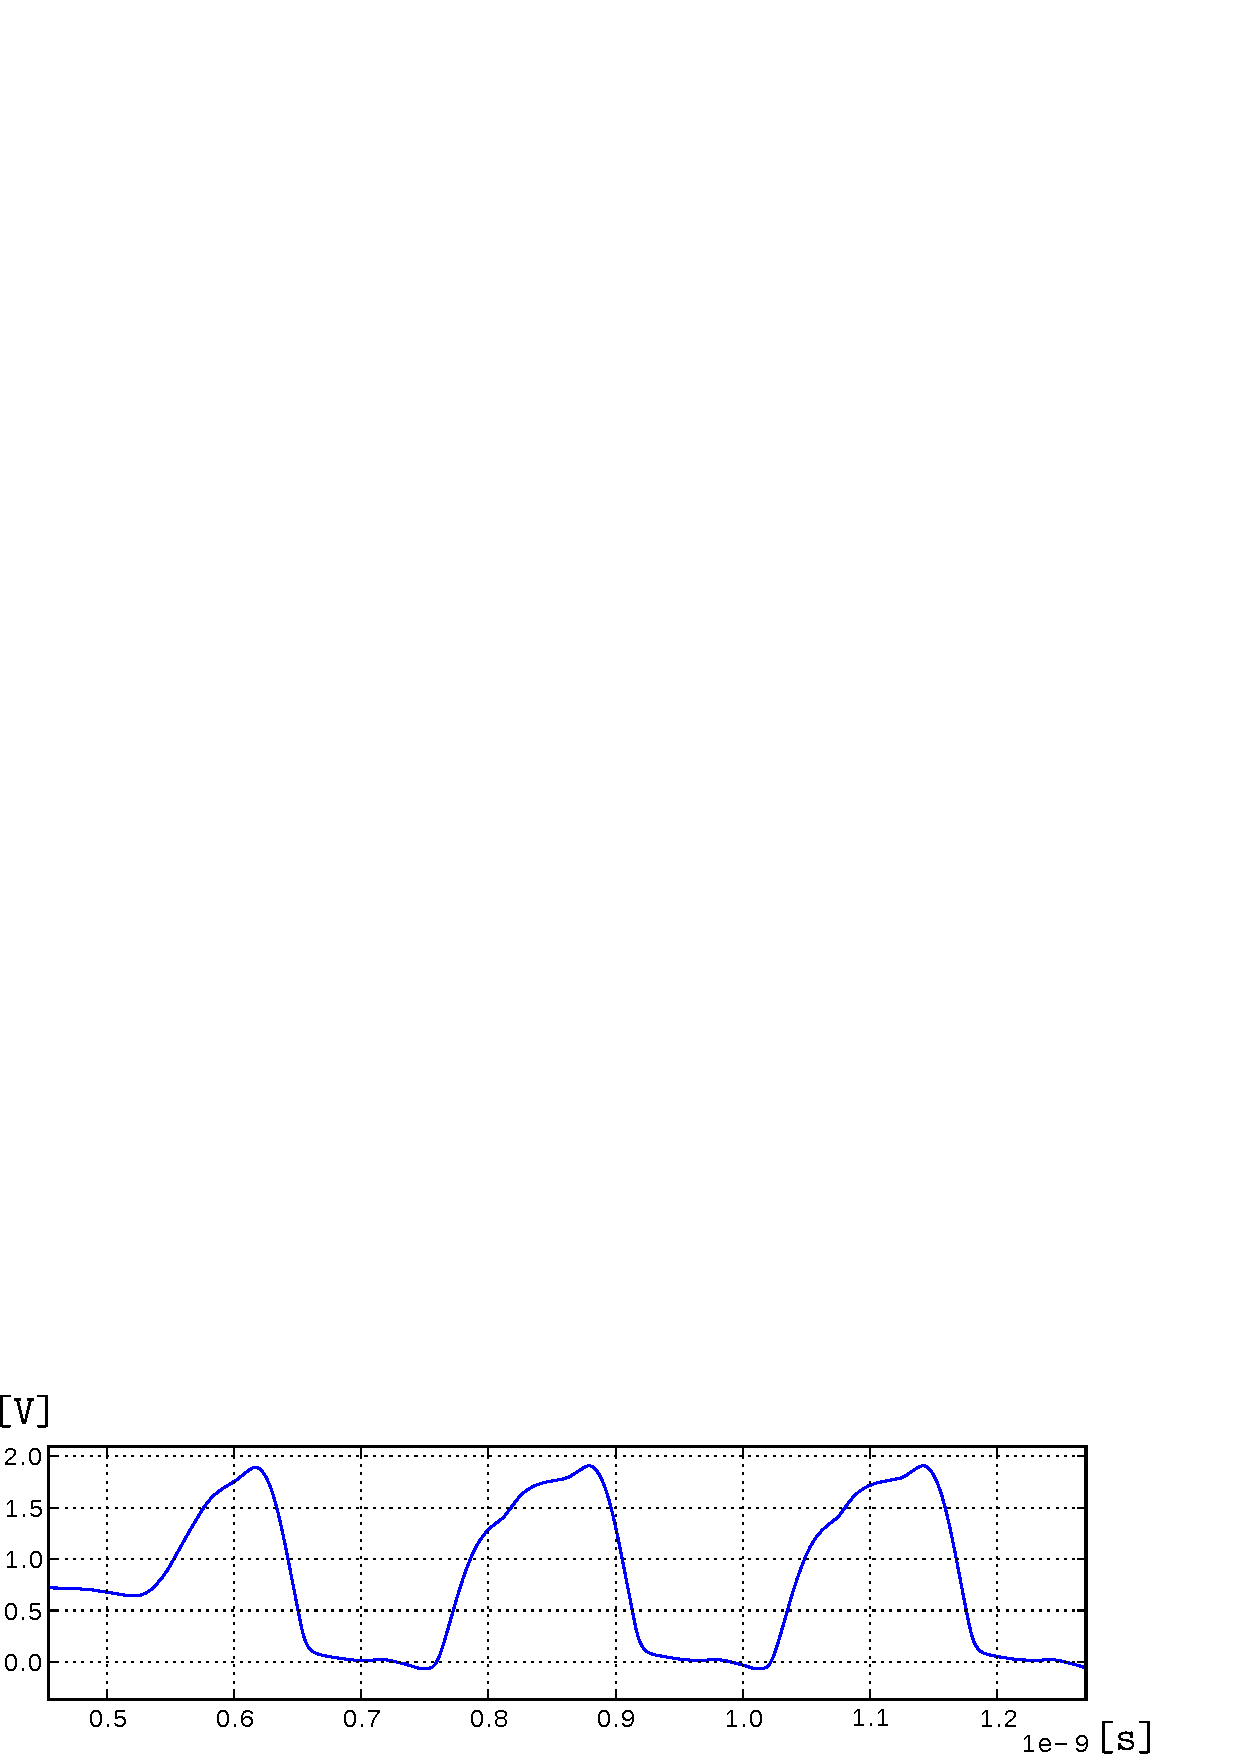
\includegraphics[scale=.3]{figuras/RO5.png}
  \caption{Layout del Oscilador anillo (N=5)}
\label{fig:RO5_lay}
\vspace{-10pt}
\end{figure}

Realizamos un oscilador anillo de 5 etapas, utilizando el inversor mas chico de nuestra librería de celdas estándard elegida. En la figura \ref{fig:RO5_lay} podemos ver el \emph{layout} que realizamos para esta prueba. Hacemos la extracción de parásitos y simulamos el circuito para obtener la forma de onda de la figura \ref{fig:RO5_wf}.

Como podemos deducir de la figura \ref{fig:RO5_wf}, el tiempo de propagación es de 32~pS, lo cual no significa que nuestros circuitos puedan correr a 31,25~GHz. Cuando medimos el tiempo de propagación usando este circuito, deberemos considerar que este es sólo una forma de comparar las tecnologías de fabricación y las topologías de las compuertas, pero de ninguna forma será la frecuencia máxima a la que pueda funcionar nuestro circuito, ya que la complejidad y cantidad de compuertas es enormemente mayor que la de un inversor. Según Rabaey\cite{rabaey2003} se puede esperar velocidades entre 50 a 100 veces mas bajas, aunque optimizando el diseño se puede lograr acercarnos un poco mas a esta frecuencia ideal. 

\begin{figure}[h!]
\vspace{-5pt}
  \centering
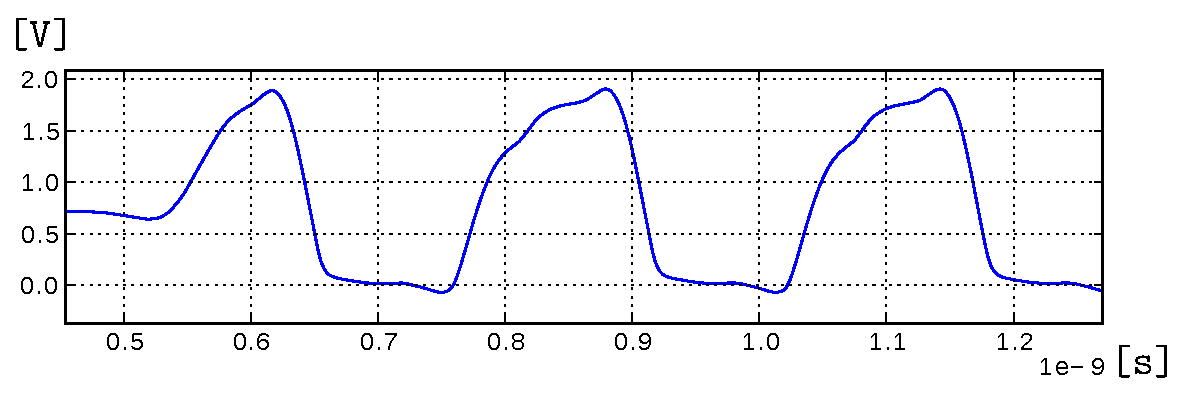
\includegraphics[scale=.6]{figuras/RO5.eps}
  \caption{Simulación con parásitos extraidos del layout de la figura \ref{fig:RO5_lay}}
\label{fig:RO5_wf}
\vspace{-10pt}
\end{figure}


\subsection{Tiempo mínimo de propagación}
t_p = 32 p

%Para simular corners: opConditions.lib


